\documentclass[../competing_bandits_with_appendix.tex]{subfiles}
\begin{document}

\subsection{Performance in Isolation, Revisited}\label{sec:revisited}


We saw in Section~\ref{sec:competition} that mean reputation trajectories do not suffice to explain the outcomes under competition. Let us provide more evidence and intuition for this.

Mean reputation trajectories are so natural that one is tempted to conjecture that they determine the outcomes under competition. More specifically:
\begin{conjecture}\label{conj:mean-trajectories}
If one algorithm's mean reputation trajectory lies above another, perhaps after some initial time interval (\eg as in Figure~\ref{prelim_means}), then the first algorithm prevails under competition, for a sufficiently large warm start $T_0$.
\end{conjecture}

However, we find a more nuanced picture. For example, in Figure \ref{fig:market_share} we see that $\DynamicGreedy$ attains a larger market share than $\DynamicEpsGreedy$ even for large warm starts. We find that this also holds for $K = 3$ arms and longer time horizons, see the supplement for more details. We conclude that Conjecture~\ref{conj:mean-trajectories} is false:

\begin{figure}[ht]
\centering
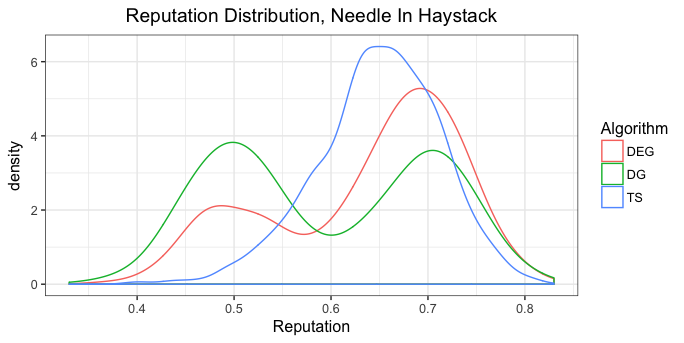
\includegraphics[scale=0.35]{ec19paper/figures/rep_distribution_nih}
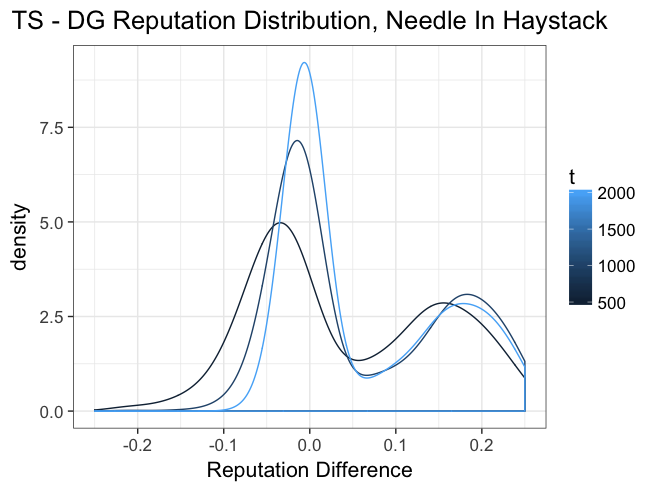
\includegraphics[scale=0.35]{ec19paper/figures/ts_dg_rep_diff_nih}
\caption{\footnotesize Needle-in-Haystack: reputation scores at $t=500$ (left), reputation difference $\Thompson - \DynamicGreedy$ (right). Both are smoothed using a kernel density estimate.}
\label{fig:rep_dist_nih}
%\caption*{\tiny{The plots contain a kernel density estimate of the reputation distribution at $t = 500$}}
\end{figure}


\begin{finding}
\textit{
Mean reputation trajectories do not suffice to explain the outcomes under competition.}
\end{finding}

To see what could go wrong with Conjecture~\ref{conj:mean-trajectories}, consider how an algorithm's reputation score is distributed at a particular time. That is, consider the empirical distribution of this score over different \MRVs.%
\footnote{Recall that each \MRV in our experimental setup comes with a separate realization table.} For concreteness, consider the Needle-in-Haystack instance at time $t=500$, plotted in Figure~\ref{fig:rep_dist_nih} (left). (The other MAB instances lead to a similar intuition.)

We see that the ``naive" algorithms $\DynamicGreedy$ and $\DynamicEpsGreedy$ have a bi-modal reputation distribution, whereas $\Thompson$ does not. The reason is that for this MAB instance, $\DynamicGreedy$ either finds the best arm and sticks to it, or gets stuck on the bad arms. In the former case \DynamicGreedy does slightly better than $\Thompson$, and in the latter case it does substantially worse. However, the mean reputation trajectory may fail to capture this complexity since it simply takes average over different \MRVs. This may be inadequate for explaining the outcome of the duopoly game, given that the latter is determined by a simple comparison between the firm's reputation scores.

To further this intuition, consider the difference in reputation scores (\emph{reputation difference}) between \Thompson and \DynamicGreedy on a particular \MRV. Let's plot the empirical distribution of the reputation difference (over the \MRVs) at a particular time point. Figure~\ref{fig:rep_dist_nih} (right) shows such plots for several time points. We observe that the distribution is skewed to the right, precisely due to the fact that $\DynamicGreedy$ either does slightly better than $\Thompson$ or does substantially worse. So, the mean is not a good measure of the central tendency of this distribution.

\OMIT{In particular, the mean reputation difference tends to overstate how well an advanced exploration algorithm (that will eventually find the best arm) should do in competition compared to a naive algorithm that may never find the best arm.}



\end{document}
%%% Local Variables:
%%% mode: latex
%%% TeX-master: "../competing_bandits"
%%% End:
